\documentclass[tikz,border=8pt]{standalone}
% Shared look for every TikZ diagram. Load with \input{../../tools/tikz-style.tex}
\usepackage[T1]{fontenc}
\usepackage{lmodern}
\renewcommand{\sfdefault}{lmr}  % diagrams use the same serif as the text
\usetikzlibrary{arrows.meta, positioning, shapes.geometric, calc, fit, backgrounds}
\definecolor{cblue}{HTML}{4C78A8}
\definecolor{corange}{HTML}{F58518}
\definecolor{cgreen}{HTML}{54A24B}
\definecolor{cred}{HTML}{E45756}
\definecolor{cpurple}{HTML}{B279A2}
\definecolor{cgrey}{HTML}{6B6B6B}
\tikzset{
  every picture/.style={font=\sffamily, line width=1.2pt},
  box/.style={draw=#1, fill=#1!12, rounded corners=4pt, align=center, inner sep=7pt, minimum height=1.1cm},
  box/.default=cgrey,
  arrow/.style={-{Stealth[length=3mm]}, draw=cgrey, line width=1.4pt},
  title/.style={font=\sffamily\bfseries\Large},
  note/.style={font=\sffamily\small, text=cgrey, align=center},
}
\AtBeginDocument{\hyphenpenalty=10000 \exhyphenpenalty=10000}

% Which model of the label, under maximum likelihood, gives which loss; and which prior, under MAP, gives which penalty.
\begin{document}
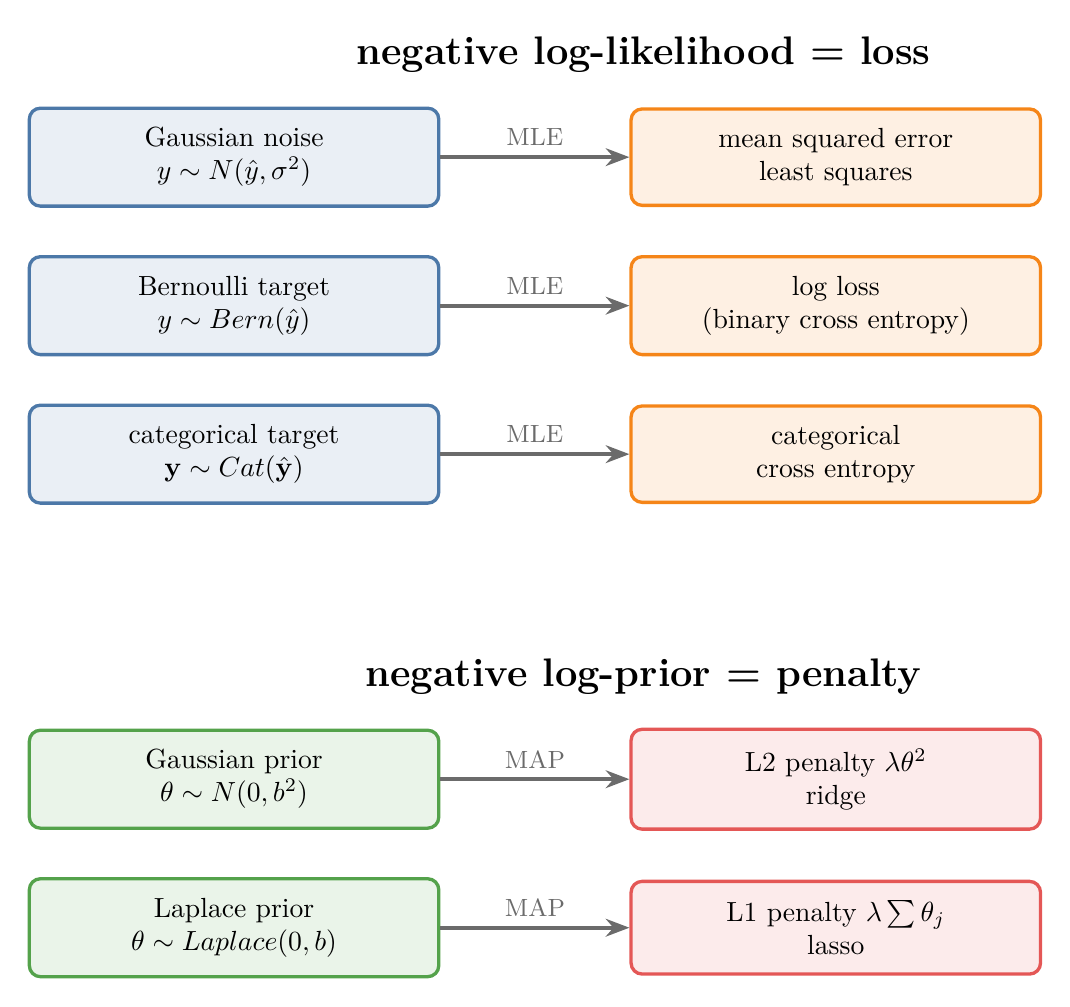
\begin{tikzpicture}[node distance=0.6cm and 1.4cm]
  \node[title] at (5.2,1.3) {negative log-likelihood = loss};
  \node[box=cblue, minimum width=5.2cm] (g) at (0,0) {Gaussian noise\\ $y \sim N(\hat y, \sigma^2)$};
  \node[box=cblue, minimum width=5.2cm, below=of g] (b) {Bernoulli target\\ $y \sim \text{Bern}(\hat y)$};
  \node[box=cblue, minimum width=5.2cm, below=of b] (c) {categorical target\\ $\mathbf{y} \sim \text{Cat}(\hat{\mathbf{y}})$};
  \node[box=corange, minimum width=5.2cm, right=2.4cm of g] (G) {mean squared error\\ least squares};
  \node[box=corange, minimum width=5.2cm, right=2.4cm of b] (B) {log loss\\ (binary cross entropy)};
  \node[box=corange, minimum width=5.2cm, right=2.4cm of c] (C) {categorical\\ cross entropy};
  \foreach \a/\z in {g/G, b/B, c/C} \draw[arrow] (\a) -- node[above, note] {MLE} (\z);
  \node[title] at (5.2,-6.6) {negative log-prior = penalty};
  \node[box=cgreen, minimum width=5.2cm] (gp) at (0,-7.9) {Gaussian prior\\ $\theta \sim N(0, b^2)$};
  \node[box=cgreen, minimum width=5.2cm, below=of gp] (lp) {Laplace prior\\ $\theta \sim \text{Laplace}(0, b)$};
  \node[box=cred, minimum width=5.2cm, right=2.4cm of gp] (R) {L2 penalty $\lambda\lVert\theta\rVert^2$\\ ridge};
  \node[box=cred, minimum width=5.2cm, right=2.4cm of lp] (L) {L1 penalty $\lambda\sum\lvert\theta_j\rvert$\\ lasso};
  \foreach \a/\z in {gp/R, lp/L} \draw[arrow] (\a) -- node[above, note] {MAP} (\z);
\end{tikzpicture}
\end{document}
